\documentclass[10pt,landscape]{article}
\usepackage[usenames,dvips,pdftex]{color}
\usepackage{multicol}
\usepackage{calc}
\usepackage{ifthen}
\usepackage[pdftex]{color,graphicx}
\usepackage[landscape]{geometry}
\usepackage{hyperref}
\hypersetup{colorlinks=true, filecolor=black, linkcolor=black, urlcolor=blue, citecolor=black}
\graphicspath{{./images/}}


% To make this come out properly in landscape mode, do one of the following
% 1.
%  pdflatex latexsheet.tex
%
% 2.
%  latex latexsheet.tex
%  dvips -P pdf  -t landscape latexsheet.dvi
%  ps2pdf latexsheet.ps


% If you're reading this, be prepared for confusion.  Making this was
% a learning experience for me, and it shows.  Much of the placement
% was hacked in; if you make it better, let me know...


% 2008-04
% Changed page margin code to use the geometry package. Also added code for
% conditional page margins, depending on paper size. Thanks to Uwe Ziegenhagen
% for the suggestions.

% 2006-08
% Made changes based on suggestions from Gene Cooperman. <gene at ccs.neu.edu>


% To Do:
% \listoffigures \listoftables
% \setcounter{secnumdepth}{0}


% This sets page margins to .5 inch if using letter paper, and to 1cm
% if using A4 paper. (This probably isn't strictly necessary.)
% If using another size paper, use default 1cm margins.
\ifthenelse{\lengthtest { \paperwidth = 11in}}
	{ \geometry{top=.5in,left=.5in,right=.5in,bottom=.5in} }
	{\ifthenelse{ \lengthtest{ \paperwidth = 297mm}}
		{\geometry{top=1cm,left=1cm,right=1cm,bottom=1cm} }
		{\geometry{top=1cm,left=1cm,right=1cm,bottom=1cm} }
	}

% Turn off header and footer
\pagestyle{empty}
 

% Redefine section commands to use less space
\makeatletter
\renewcommand{\section}{\@startsection{section}{1}{0mm}%
                                {-1ex plus -.5ex minus -.2ex}%
                                {0.5ex plus .2ex}%x
                                {\normalfont\large\bfseries}}
\renewcommand{\subsection}{\@startsection{subsection}{2}{0mm}%
                                {-1explus -.5ex minus -.2ex}%
                                {0.5ex plus .2ex}%
                                {\normalfont\normalsize\bfseries}}
\renewcommand{\subsubsection}{\@startsection{subsubsection}{3}{0mm}%
                                {-1ex plus -.5ex minus -.2ex}%
                                {1ex plus .2ex}%
                                {\normalfont\small\bfseries}}
\makeatother

% Define BibTeX command
\def\BibTeX{{\rm B\kern-.05em{\sc i\kern-.025em b}\kern-.08em
    T\kern-.1667em\lower.7ex\hbox{E}\kern-.125emX}}

% Don't print section numbers
\setcounter{secnumdepth}{0}


\setlength{\parindent}{0pt}
\setlength{\parskip}{0pt plus 0.5ex}


% -----------------------------------------------------------------------

\begin{document}

\raggedright
\footnotesize
\begin{multicols}{3}


% multicol parameters
% These lengths are set only within the two main columns
%\setlength{\columnseprule}{0.25pt}
\setlength{\premulticols}{1pt}
\setlength{\postmulticols}{1pt}
\setlength{\multicolsep}{1pt}
\setlength{\columnsep}{2pt}

\begin{center}
     \Large{\textbf{ROS Cheat Sheet}} \\
\end{center}
\newlength{\MyLen}
\settowidth{\MyLen}{\texttt{letterpaper}/\texttt{a4paper} \ }

%\section{Filesystem Concepts}
%\begin{tabular}{@{}p{\the\MyLen}%
 %               @{}p{\linewidth-\the\MyLen}@{}}
%\texttt{\href{http://www.ros.org/wiki/Packages}{package}}   & The lowest level of ROS software organization. \\
%\texttt{\href{http://www.ros.org/wiki/Manifest}{manifest}}  & Description of a ROS package. \\
%\texttt{\href{http://www.ros.org/wiki/Stack}{stack}} & Collections of ROS packages that form a higher-level library. \\
%\texttt{\href{http://www.ros.org/wiki/Stack Manifest}{stack manifest}}  & Description of a ROS stack.
%\end{tabular}

\section{Filesystem Command-line Tools}
\begin{tabular}{@{}p{\the\MyLen}%
                @{}p{\linewidth-\the\MyLen}@{}}
\texttt{\href{http://www.ros.org/wiki/rospack}{rospack}}/\texttt{rosstack} & A tool inspecting \href{http://www.ros.org/wiki/Packages}{packages}/\href{http://www.ros.org/wiki/Stack}{stacks}. \\
\texttt{roscd} & Changes directories to a package or stack. \\
\texttt{rosls} & Lists package or stack information. \\
\texttt{\href{http://www.ros.org/wiki/roscreate}{roscreate}-pkg} & Creates a new ROS package. \\
\texttt{\href{http://www.ros.org/wiki/roscreate}{roscreate}-stack} & Creates a new ROS stack.\\
\texttt{\href{http://www.ros.org/wiki/rosdep}{rosdep}} & Installs ROS package system dependencies.\\
\texttt{\href{http://www.ros.org/wiki/rosmake}{rosmake}} & Builds a ROS package.\\
\texttt{\href{http://www.ros.org/wiki/rosmsg}{rosmsg}}/\texttt{rossrv} & Displays information about ROS \href{http://www.ros.org/wiki/msg}{message}/\href{http://www.ros.org/wiki/srv}{service} types .
\end{tabular}

\begin{tabbing}
Us\=age:\\
\> \texttt{\$ rospack find [package]}\\  
\> \texttt{\$ roscd [package[/subdir]]}\\
\> \texttt{\$ rosls [package[/subdir]]}\\
\> \texttt{\$ roscreate-pkg [package\_name]}\\
\> \texttt{\$ rosmake [package]}\\
\> \texttt{\$ rosdep install [package]}\\
\> \texttt{\$ rosmsg show [message type]}
\end{tabbing}

%\section{Graph Concepts}
%\settowidth{\MyLen}{\texttt{multicol} }
%\begin{tabular}{@{}p{\the\MyLen}%
%                @{}p{\linewidth-\the\MyLen}@{}}
%\texttt{\href{http://www.ros.org/wiki/Master}{master}}   & Provides naming and registration services to ROS nodes. \\
%\texttt{\href{http://www.ros.org/wiki/Nodes}{nodes}}   & Process that performs computation. \\
%\texttt{\href{http://www.ros.org/wiki/Topics}{topics}}  & Named buses over which ROS nodes exchange ROS messages. \\
%\texttt{\href{http://www.ros.org/wiki/Messages}{messages}} & A data structure comprising typed fields. \\
%\texttt{\href{http://www.ros.org/wiki/Services}{services}}  & A data structure comprising typed fields with a request and reply.\\
%\texttt{\href{http://www.ros.org/wiki/Parameter Server}{parameter server}}  & A shared multi-variate dictionary where ROS nodes can store and retrieve parameters at runtime.
%\end{tabular}

\section{Graph Command-line Tools}
\subsection{\href{http://www.ros.org/wiki/roscore}{roscore}}
A collection of \href{http://www.ros.org/wiki/Nodes}{nodes} and programs that are pre-requisites of a ROS-based system. You must have a roscore running in order for ROS nodes to communicate.\\
\begin{tabbing}
ro\=score is currently defined as:\\
\> \texttt{\href{http://www.ros.org/wiki/Master}{master}}\\
\> \texttt{\href{http://www.ros.org/wiki/Parameter Server}{parameter server}}\\
\> \texttt{\href{http://www.ros.org/wiki/rosout}{rosout}}
\end{tabbing}
\begin{tabbing}
Us\=age:\\
\> \texttt{\$ roscore}
\end{tabbing}

\subsection{\href{http://www.ros.org/wiki/rosgraph}{rxgraph}}
Displays a graph of the ROS nodes that are currently running, as well as the ROS topics that connect them.\\
\vspace{2.5 mm}
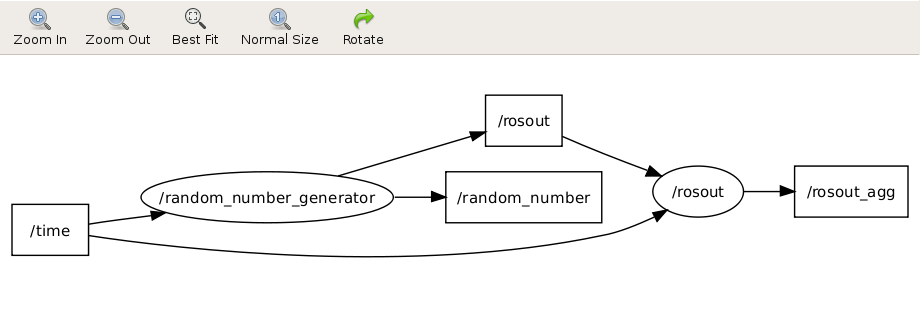
\includegraphics[width=\columnwidth]{rxgraph.png}
\begin{tabbing}
Us\=age:\\
\> \texttt{\$ rxgraph}
\end{tabbing}

\subsection{\href{http://www.ros.org/wiki/rosnode}{rosnode}}
Displays debugging information about ROS nodes, including publications, subscriptions and connections.\\
\vspace{2.5 mm}
Current list of supported commands: \\ 
\begin{tabular}{@{}p{\the\MyLen}%
                @{}p{\linewidth-\the\MyLen}@{}}
\texttt{rosnode ping}    & Test connectivity to node. \\
\texttt{rosnode list}    & List active nodes. \\
\texttt{rosnode info}    & Print information about a node. \\
\texttt{rosnode machine} & List nodes running on a particular machine. \\
\texttt{rosnode kill}    & Kills a running node. 
\end{tabular}
\begin{tabbing}
Us\=age:\\
\> \texttt{\$ rosnode [command] -h}
\end{tabbing}
\begin{tabbing}
E\=x\=amples:\\
\> Kill all nodes:\\
\> \> \texttt{\$ rosnode kill -a}\\
\> List nodes on a machine:\\
\> \> \texttt{\$ rosnode machine aqy.local}\\
\> Ping all nodes:\\
\> \> \texttt{\$ rosnode ping --all} 
\end{tabbing}

\subsection{\href{http://www.ros.org/wiki/rostopic}{rostopic}}
A tool for displaying debug information about ROS \href{http://www.ros.org/wiki/Topics}{topics}, including publishers, subscribers, publishing rate, and messages.\\
\vspace{2.5 mm}
Current list of supported commands: \\ 
\begin{tabular}{@{}p{\the\MyLen}%
                @{}p{\linewidth-\the\MyLen}@{}}
\texttt{rostopic bw}   & Display bandwidth used by topic. \\
\texttt{rostopic echo}   & Print messages to screen. \\
\texttt{rostopic hz}   & Display publishing rate of topic. \\
\texttt{rostopic list}   & Print information about active topics. \\
\texttt{rostopic pub}   & Publish data to topic. \\
\texttt{rostopic type}   & Print topic type. \\
\texttt{rostopic find}   & Find topics by type. 
\end{tabular}
\begin{tabbing}
Us\=age:\\
\> \texttt{\$ rostopic [command] -h}
\end{tabbing}

\begin{tabbing}
E\=x\=amples:\\
\> Publish hello at 10 Hz:\\
\> \>\texttt{\$ rostopic pub -r 10 /topic\_name std\_msgs/String hello}\\
\> Clear the screen after each message is published:\\
\> \>\texttt{\$ rostopic echo -c /topic\_name}\\
\> Display messages that match a given Python expression:\\
\> \>\texttt{\$ rostopic echo --filter "m.data=='foo'"  /topic\_name}\\
\> Pipe the output of rostopic to rosmsg to view the msg type:\\
\> \>\texttt{\$ rostopic type /topic\_name | rosmsg show}
\end{tabbing}

\subsection{\href{http://www.ros.org/wiki/roslaunch}{roslaunch}}
Starts ROS nodes locally and remotely via SSH, as well as setting parameters on the parameter server.\\
\begin{tabbing}
Us\=age:\\
\> \texttt{\$ roslaunch [package\_name] [file\_name]}
\end{tabbing}


\settowidth{\MyLen}{\texttt{.author.text.} }
\begin{tabular}{@{}p{\the\MyLen}%
                @{}p{\linewidth-\the\MyLen}@{}}
\verb!\author{!\textit{text}\verb!}! & Author of document. \\
\verb!\title{!\textit{text}\verb!}!  & Title of document. \\
\verb!\date{!\textit{text}\verb!}!   & Date. \\
\end{tabular}

These commands go before \verb!\begin{document}!.  The declaration
\verb!\maketitle! goes at the top of the document.

\section{Document structure}
\begin{multicols}{2}
\verb!\part{!\textit{title}\verb!}!  \\
\verb!\chapter{!\textit{title}\verb!}!  \\
\verb!\section{!\textit{title}\verb!}!  \\
\verb!\subsection{!\textit{title}\verb!}!  \\
\verb!\subsubsection{!\textit{title}\verb!}!  \\
\verb!\paragraph{!\textit{title}\verb!}!  \\
\verb!\subparagraph{!\textit{title}\verb!}!
\end{multicols}
{\raggedright
Section commands can be followed with an \texttt{*}, like
\verb!\section*{!\textit{title}\verb!}!, to supress heading
numbers. \verb!\setcounter{secnumdepth}{!$x$\verb!}! supresses heading
numbers of depth $>x$, where \verb!chapter! has depth 0.
}

\subsection{Text environments}
\settowidth{\MyLen}{\texttt{.begin.quotation.}}
\begin{tabular}{@{}p{\the\MyLen}%
                @{}p{\linewidth-\the\MyLen}@{}}
\verb!\begin{comment}!    &  Comment block (not printed). \\
\verb!\begin{quote}!      &  Indented quotation block. \\
\verb!\begin{quotation}!  &  Like \texttt{quote} with indented paragraphs. \\
\verb!\begin{verse}!      &  Quotation block for verse.
\end{tabular}

\subsection{Lists}
\settowidth{\MyLen}{\texttt{.begin.description.}}
\begin{tabular}{@{}p{\the\MyLen}%
                @{}p{\linewidth-\the\MyLen}@{}}
\verb!\begin{enumerate}!        &  Numbered list. \\
\verb!\begin{itemize}!          &  Bulleted list. \\
\verb!\begin{description}!      &  Description list. \\
\verb!\item! \textit{text}      &  Add an item. \\
\verb!\item[!\textit{x}\verb!]! \textit{text}
                                &  Use \textit{x} instead of normal
                        bullet or number.  Required for descriptions. \\
\end{tabular}




\subsection{References}
\settowidth{\MyLen}{\texttt{.pageref.marker..}}
\begin{tabular}{@{}p{\the\MyLen}%
                @{}p{\linewidth-\the\MyLen}@{}}
\verb!\label{!\textit{marker}\verb!}!   &  Set a marker for cross-reference, 
                          often of the form \verb!\label{sec:item}!. \\
\verb!\ref{!\textit{marker}\verb!}!   &  Give section/body number of marker. \\
\verb!\pageref{!\textit{marker}\verb!}! &  Give page number of marker. \\
\verb!\footnote{!\textit{text}\verb!}!  &  Print footnote at bottom of page. \\
\end{tabular}


\subsection{Floating bodies}
\settowidth{\MyLen}{\texttt{.begin.equation..place.}}
\begin{tabular}{@{}p{\the\MyLen}%
                @{}p{\linewidth-\the\MyLen}@{}}
\verb!\begin{table}[!\textit{place}\verb!]!     &  Add numbered table. \\
\verb!\begin{figure}[!\textit{place}\verb!]!    &  Add numbered figure. \\
\verb!\begin{equation}[!\textit{place}\verb!]!  &  Add numbered equation. \\
\verb!\caption{!\textit{text}\verb!}!           &  Caption for the body. \\
\end{tabular}

The \textit{place} is a list valid placements for the body.  \texttt{t}=top,
\texttt{h}=here, \texttt{b}=bottom, \texttt{p}=separate page, \texttt{!}=place even if ugly.  Captions and label markers should be within the environment.

%---------------------------------------------------------------------------

\section{Text properties}

\subsection{Font face}
\newcommand{\FontCmd}[3]{\PBS\verb!\#1{!\textit{text}\verb!}!  \> %
                         \verb!{\#2 !\textit{text}\verb!}! \> %
                         \#1{#3}}
\begin{tabular}{@{}l@{}l@{}l@{}}
\textit{Command} & \textit{Declaration} & \textit{Effect} \\
\verb!\textrm{!\textit{text}\verb!}!                    & %
        \verb!{\rmfamily !\textit{text}\verb!}!               & %
        \textrm{Roman family} \\
\verb!\textsf{!\textit{text}\verb!}!                    & %
        \verb!{\sffamily !\textit{text}\verb!}!               & %
        \textsf{Sans serif family} \\
\verb!\texttt{!\textit{text}\verb!}!                    & %
        \verb!{\ttfamily !\textit{text}\verb!}!               & %
        \texttt{Typewriter family} \\
\verb!\textmd{!\textit{text}\verb!}!                    & %
        \verb!{\mdseries !\textit{text}\verb!}!               & %
        \textmd{Medium series} \\
\verb!\textbf{!\textit{text}\verb!}!                    & %
        \verb!{\bfseries !\textit{text}\verb!}!               & %
        \textbf{Bold series} \\
\verb!\textup{!\textit{text}\verb!}!                    & %
        \verb!{\upshape !\textit{text}\verb!}!               & %
        \textup{Upright shape} \\
\verb!\textit{!\textit{text}\verb!}!                    & %
        \verb!{\itshape !\textit{text}\verb!}!               & %
        \textit{Italic shape} \\
\verb!\textsl{!\textit{text}\verb!}!                    & %
        \verb!{\slshape !\textit{text}\verb!}!               & %
        \textsl{Slanted shape} \\
\verb!\textsc{!\textit{text}\verb!}!                    & %
        \verb!{\scshape !\textit{text}\verb!}!               & %
        \textsc{Small Caps shape} \\
\verb!\emph{!\textit{text}\verb!}!                      & %
        \verb!{\em !\textit{text}\verb!}!               & %
        \emph{Emphasized} \\
\verb!\textnormal{!\textit{text}\verb!}!                & %
        \verb!{\normalfont !\textit{text}\verb!}!       & %
        \textnormal{Document font} \\
\verb!\underline{!\textit{text}\verb!}!                 & %
                                                        & %
        \underline{Underline}
\end{tabular}

The command (t\textit{tt}t) form handles spacing better than the
declaration (t{\itshape tt}t) form.

\subsection{Font size}
\setlength{\columnsep}{14pt} % Need to move columns apart a little
\begin{multicols}{2}
\begin{tabbing}
\verb!\footnotesize!          \= \kill
\verb!\tiny!                  \>  \tiny{tiny} \\
\verb!\scriptsize!            \>  \scriptsize{scriptsize} \\
\verb!\footnotesize!          \>  \footnotesize{footnotesize} \\
\verb!\small!                 \>  \small{small} \\
\verb!\normalsize!            \>  \normalsize{normalsize} \\
\verb!\large!                 \>  \large{large} \\
\verb!\Large!                 \=  \Large{Large} \\  % Tab hack for new column
\verb!\LARGE!                 \>  \LARGE{LARGE} \\
\verb!\huge!                  \>  \huge{huge} \\
\verb!\Huge!                  \>  \Huge{Huge}
\end{tabbing}
\end{multicols}
\setlength{\columnsep}{1pt} % Set column separation back

These are declarations and should be used in the form
\verb!{\small! \ldots\verb!}!, or without braces to affect the entire
document.


\subsection{Verbatim text}

\settowidth{\MyLen}{\texttt{.begin.verbatim..} }
\begin{tabular}{@{}p{\the\MyLen}%
                @{}p{\linewidth-\the\MyLen}@{}}
\verb@\begin{verbatim}@ & Verbatim environment. \\
\verb@\begin{verbatim*}@ & Spaces are shown as \verb*@ @. \\
\verb@\verb!text!@ & Text between the delimiting characters (in this case %
                      `\texttt{!}') is verbatim.
\end{tabular}


\subsection{Justification}
\begin{tabular}{@{}ll@{}}
\textit{Environment}  &  \textit{Declaration}  \\
\verb!\begin{center}!      & \verb!\centering!  \\
\verb!\begin{flushleft}!  & \verb!\raggedright! \\
\verb!\begin{flushright}! & \verb!\raggedleft!  \\
\end{tabular}

\subsection{Miscellaneous}
\verb!\linespread{!$x$\verb!}! changes the line spacing by the
multiplier $x$.





\section{Text-mode symbols}

\subsection{Symbols}
\begin{tabular}{@{}l@{\hspace{1em}}l@{\hspace{2em}}l@{\hspace{1em}}l@{\hspace{2em}}l@{\hspace{1em}}l@{\hspace{2em}}l@{\hspace{1em}}l@{}}
\&              &  \verb!\&! &
\_              &  \verb!\_! &
\ldots          &  \verb!\ldots! &
\textbullet     &  \verb!\textbullet! \\
\$              &  \verb!\$! &
\^{}            &  \verb!\^{}! &
\textbar        &  \verb!\textbar! &
\textbackslash  &  \verb!\textbackslash! \\
\%              &  \verb!\%! &
\~{}            &  \verb!\~{}! &
\#              &  \verb!\#! &
\S              &  \verb!\S! \\
\end{tabular}

\subsection{Accents}
\begin{tabular}{@{}l@{\ }l|l@{\ }l|l@{\ }l|l@{\ }l|l@{\ }l@{}}
\`o   & \verb!\`o! &
\'o   & \verb!\'o! &
\^o   & \verb!\^o! &
\~o   & \verb!\~o! &
\=o   & \verb!\=o! \\
\.o   & \verb!\.o! &
\"o   & \verb!\"o! &
\c o  & \verb!\c o! &
\v o  & \verb!\v o! &
\H o  & \verb!\H o! \\
\c c  & \verb!\c c! &
\d o  & \verb!\d o! &
\b o  & \verb!\b o! &
\t oo & \verb!\t oo! &
\oe   & \verb!\oe! \\
\OE   & \verb!\OE! &
\ae   & \verb!\ae! &
\AE   & \verb!\AE! &
\aa   & \verb!\aa! &
\AA   & \verb!\AA! \\
\o    & \verb!\o! &
\O    & \verb!\O! &
\l    & \verb!\l! &
\L    & \verb!\L! &
\i    & \verb!\i! \\
\j    & \verb!\j! &
!`    & \verb!~`! &
?`    & \verb!?`! &
\end{tabular}


\subsection{Delimiters}
\begin{tabular}{@{}l@{\ }ll@{\ }ll@{\ }ll@{\ }ll@{\ }ll@{\ }l@{}}
`       & \verb!`!  &
``      & \verb!``! &
\{      & \verb!\{! &
\lbrack & \verb![! &
(       & \verb!(! &
\textless  &  \verb!\textless! \\
'       & \verb!'!  &
''      & \verb!''! &
\}      & \verb!\}! &
\rbrack & \verb!]! &
)       & \verb!)! &
\textgreater  &  \verb!\textgreater! \\
\end{tabular}

\subsection{Dashes}
\begin{tabular}{@{}llll@{}}
\textit{Name} & \textit{Source} & \textit{Example} & \textit{Usage} \\
hyphen  & \verb!-!   & X-ray          & In words. \\
en-dash & \verb!--!  & 1--5           & Between numbers. \\
em-dash & \verb!---! & Yes---or no?    & Punctuation.
\end{tabular}


\subsection{Line and page breaks}
\settowidth{\MyLen}{\texttt{.pagebreak} }
\begin{tabular}{@{}p{\the\MyLen}%
                @{}p{\linewidth-\the\MyLen}@{}}
\verb!\\!          &  Begin new line without new paragraph.  \\
\verb!\\*!         &  Prohibit pagebreak after linebreak. \\
\verb!\kill!       &  Don't print current line. \\
\verb!\pagebreak!  &  Start new page. \\
\verb!\noindent!   &  Do not indent current line.
\end{tabular}


\subsection{Miscellaneous}
\settowidth{\MyLen}{\texttt{.rule.w..h.} }
\begin{tabular}{@{}p{\the\MyLen}%
                @{}p{\linewidth-\the\MyLen}@{}}
\verb!\today!  &  \today. \\
\verb!$\sim$!  &  Prints $\sim$ instead of \verb!\~{}!, which makes \~{}. \\
\verb!~!       &  Space, disallow linebreak (\verb!W.J.~Clinton!). \\
\verb!\@.!     &  Indicate that the \verb!.! ends a sentence when following
                        an uppercase letter. \\
\verb!\hspace{!$l$\verb!}! & Horizontal space of length $l$
                                (Ex: $l=\mathtt{20pt}$). \\
\verb!\vspace{!$l$\verb!}! & Vertical space of length $l$. \\
\verb!\rule{!$w$\verb!}{!$h$\verb!}! & Line of width $w$ and height $h$. \\
\end{tabular}



\section{Tabular environments}

\subsection{\texttt{tabbing} environment}
\begin{tabular}{@{}l@{\hspace{1.5ex}}l@{\hspace{10ex}}l@{\hspace{1.5ex}}l@{}}
\verb!\=!  &   Set tab stop. &
\verb!\>!  &   Go to tab stop.
\end{tabular}

Tab stops can be set on ``invisible'' lines with \verb!\kill!
at the end of the line.  Normally \verb!\\! is used to separate lines.


\subsection{\texttt{tabular} environment}
\verb!\begin{array}[!\textit{pos}\verb!]{!\textit{cols}\verb!}!   \\
\verb!\begin{tabular}[!\textit{pos}\verb!]{!\textit{cols}\verb!}! \\
\verb!\begin{tabular*}{!\textit{width}\verb!}[!\textit{pos}\verb!]{!\textit{cols}\verb!}!


\subsubsection{\texttt{tabular} column specification}
\settowidth{\MyLen}{\texttt{p}\{\textit{width}\} \ }
\begin{tabular}{@{}p{\the\MyLen}@{}p{\linewidth-\the\MyLen}@{}}
\texttt{l}    &   Left-justified column.  \\
\texttt{c}    &   Centered column.  \\
\texttt{r}    &   Right-justified column. \\
\verb!p{!\textit{width}\verb!}!  &  Same as %
                              \verb!\parbox[t]{!\textit{width}\verb!}!. \\ 
\verb!@{!\textit{decl}\verb!}!   &  Insert \textit{decl} instead of
                                    inter-column space. \\
\verb!|!      &   Inserts a vertical line between columns. 
\end{tabular}


\subsubsection{\texttt{tabular} elements}
\settowidth{\MyLen}{\texttt{.cline.x-y..}}
\begin{tabular}{@{}p{\the\MyLen}@{}p{\linewidth-\the\MyLen}@{}}
\verb!\hline!           &  Horizontal line between rows.  \\
\verb!\cline{!$x$\verb!-!$y$\verb!}!  &
                        Horizontal line across columns $x$ through $y$. \\
\verb!\multicolumn{!\textit{n}\verb!}{!\textit{cols}\verb!}{!\textit{text}\verb!}! \\
        &  A cell that spans \textit{n} columns, with \textit{cols} column specification.
\end{tabular}


\section{Math mode}
To use math mode, surround text with \texttt{\$} or use
\verb!\begin{equation}!.

\begin{tabular}{@{}l@{\hspace{1em}}l@{\hspace{2em}}l@{\hspace{1em}}l@{}}
Superscript$^{x}$       &
\verb!^{x}!             &  
Subscript$_{x}$         &
\verb!_{x}!             \\  
$\frac{x}{y}$           &
\verb!\frac{x}{y}!      &  
$\sum_{k=1}^n$          &
\verb!\sum_{k=1}^n!     \\  
$\sqrt[n]{x}$           &
\verb!\sqrt[n]{x}!      &  
$\prod_{k=1}^n$         &
\verb!\prod_{k=1}^n!    \\ 
\end{tabular}

\subsection{Math-mode symbols}

% The ordering of these symbols is slightly odd.  This is because I had to put all the
% long pieces of text in the same column (the right) for it all to fit properly.
% Otherwise, it wouldn't be possible to fit four columns of symbols here.

\begin{tabular}{@{}l@{\hspace{1ex}}l@{\hspace{1em}}l@{\hspace{1ex}}l@{\hspace{1em}}l@{\hspace{1ex}} l@{\hspace{1em}}l@{\hspace{1ex}}l@{}}
$\leq$          &  \verb!\leq!  &
$\geq$          &  \verb!\geq!  &
$\neq$          &  \verb!\neq!  &
$\approx$       &  \verb!\approx!  \\
$\times$        &  \verb!\times!  &
$\div$          &  \verb!\div!  &
$\pm$           & \verb!\pm!  &
$\cdot$         &  \verb!\cdot!  \\
$^{\circ}$      & \verb!^{\circ}! &
$\circ$         &  \verb!\circ!  &
$\prime$        & \verb!\prime!  &
$\cdots$        &  \verb!\cdots!  \\
$\infty$        & \verb!\infty!  &
$\neg$          & \verb!\neg!  &
$\wedge$        & \verb!\wedge!  &
$\vee$          & \verb!\vee!  \\
$\supset$       & \verb!\supset!  &
$\forall$       & \verb!\forall!  &
$\in$           & \verb!\in!  &
$\rightarrow$   &  \verb!\rightarrow! \\
$\subset$       & \verb!\subset!  &
$\exists$       & \verb!\exists!  &
$\notin$        & \verb!\notin!  &
$\Rightarrow$   &  \verb!\Rightarrow! \\
$\cup$          & \verb!\cup!  &
$\cap$          & \verb!\cap!  &
$\mid$          & \verb!\mid!  &
$\Leftrightarrow$   &  \verb!\Leftrightarrow! \\
$\dot a$        & \verb!\dot a!  &
$\hat a$        & \verb!\hat a!  &
$\bar a$        & \verb!\bar a!  &
$\tilde a$      & \verb!\tilde a!  \\

$\alpha$        &  \verb!\alpha!  &
$\beta$         &  \verb!\beta!  &
$\gamma$        &  \verb!\gamma!  &
$\delta$        &  \verb!\delta!  \\
$\epsilon$      &  \verb!\epsilon!  &
$\zeta$         &  \verb!\zeta!  &
$\eta$          &  \verb!\eta!  &
$\varepsilon$   &  \verb!\varepsilon!  \\
$\theta$        &  \verb!\theta!  &
$\iota$         &  \verb!\iota!  &
$\kappa$        &  \verb!\kappa!  &
$\vartheta$     &  \verb!\vartheta!  \\
$\lambda$       &  \verb!\lambda!  &
$\mu$           &  \verb!\mu!  &
$\nu$           &  \verb!\nu!  &
$\xi$           &  \verb!\xi!  \\
$\pi$           &  \verb!\pi!  &
$\rho$          &  \verb!\rho!  &
$\sigma$        &  \verb!\sigma!  &
$\tau$          &  \verb!\tau!  \\
$\upsilon$      &  \verb!\upsilon!  &
$\phi$          &  \verb!\phi!  &
$\chi$          &  \verb!\chi!  &
$\psi$          &  \verb!\psi!  \\
$\omega$        &  \verb!\omega!  &
$\Gamma$        &  \verb!\Gamma!  &
$\Delta$        &  \verb!\Delta!  &
$\Theta$        &  \verb!\Theta!  \\
$\Lambda$       &  \verb!\Lambda!  &
$\Xi$           &  \verb!\Xi!  &
$\Pi$           &  \verb!\Pi!  &
$\Sigma$        &  \verb!\Sigma!  \\
$\Upsilon$      &  \verb!\Upsilon!  &
$\Phi$          &  \verb!\Phi!  &
$\Psi$          &  \verb!\Psi!  &
$\Omega$        &  \verb!\Omega!  
\end{tabular}
\footnotesize

%\subsection{Special symbols}
%\begin{tabular}{@{}ll@{}}
%$^{\circ}$  &  \verb!^{\circ}! Ex: $22^{\circ}\mathrm{C}$: \verb!$22^{\circ}\mathrm{C}$!.
%\end{tabular}

\section{Bibliography and citations}
When using \BibTeX, you need to run \texttt{latex}, \texttt{bibtex},
and \texttt{latex} twice more to resolve dependencies.

\subsection{Citation types}
\settowidth{\MyLen}{\texttt{.shortciteN.key..}}
\begin{tabular}{@{}p{\the\MyLen}@{}p{\linewidth-\the\MyLen}@{}}
\verb!\cite{!\textit{key}\verb!}!       &
        Full author list and year. (Watson and Crick 1953) \\
\verb!\citeA{!\textit{key}\verb!}!      &
        Full author list. (Watson and Crick) \\
\verb!\citeN{!\textit{key}\verb!}!      &
        Full author list and year. Watson and Crick (1953) \\
\verb!\shortcite{!\textit{key}\verb!}!  &
        Abbreviated author list and year. ? \\
\verb!\shortciteA{!\textit{key}\verb!}! &
        Abbreviated author list. ? \\
\verb!\shortciteN{!\textit{key}\verb!}! &
        Abbreviated author list and year. ? \\
\verb!\citeyear{!\textit{key}\verb!}!   &
        Cite year only. (1953) \\
\end{tabular}

All the above have an \texttt{NP} variant without parentheses;
Ex. \verb!\citeNP!.


\subsection{\BibTeX\ entry types}
\settowidth{\MyLen}{\texttt{.mastersthesis.}}
\begin{tabular}{@{}p{\the\MyLen}@{}p{\linewidth-\the\MyLen}@{}}
\verb!@article!         &  Journal or magazine article. \\
\verb!@book!            &  Book with publisher. \\
\verb!@booklet!         &  Book without publisher. \\
\verb!@conference!      &  Article in conference proceedings. \\
\verb!@inbook!          &  A part of a book and/or range of pages. \\
\verb!@incollection!    &  A part of book with its own title. \\
%\verb!@manual!          &  Technical documentation. \\
%\verb!@mastersthesis!   &  Master's thesis. \\
\verb!@misc!            &  If nothing else fits. \\
\verb!@phdthesis!       &  PhD. thesis. \\
\verb!@proceedings!     &  Proceedings of a conference. \\
\verb!@techreport!      &  Tech report, usually numbered in series. \\
\verb!@unpublished!     &  Unpublished. \\
\end{tabular}

\subsection{\BibTeX\ fields}
\settowidth{\MyLen}{\texttt{organization.}}
\begin{tabular}{@{}p{\the\MyLen}@{}p{\linewidth-\the\MyLen}@{}}
\verb!address!         &  Address of publisher.  Not necessary for major
                                publishers.  \\
\verb!author!           &  Names of authors, of format .... \\
\verb!booktitle!        &  Title of book when part of it is cited. \\
\verb!chapter!          &  Chapter or section number. \\
\verb!edition!          &  Edition of a book. \\
\verb!editor!           &  Names of editors. \\
\verb!institution!      &  Sponsoring institution of tech.\ report. \\
\verb!journal!          &  Journal name. \\
\verb!key!              &  Used for cross ref.\ when no author. \\
\verb!month!            &  Month published. Use 3-letter abbreviation. \\
\verb!note!             &  Any additional information. \\
\verb!number!           &  Number of journal or magazine. \\
\verb!organization!     &  Organization that sponsors a conference. \\
\verb!pages!            &  Page range (\verb!2,6,9--12!). \\
\verb!publisher!        &  Publisher's name. \\
\verb!school!           &  Name of school (for thesis). \\
\verb!series!           &  Name of series of books. \\
\verb!title!            &  Title of work. \\
\verb!type!             &  Type of tech.\ report, ex. ``Research Note''. \\
\verb!volume!           &  Volume of a journal or book. \\
\verb!year!             &  Year of publication. \\
\end{tabular}
Not all fields need to be filled.  See example below.

\subsection{Common \BibTeX\ style files}
\begin{tabular}{@{}l@{\hspace{1em}}l@{\hspace{3em}}l@{\hspace{1em}}l@{}}
\verb!abbrv!    &  Standard &
\verb!abstract! &  \texttt{alpha} with abstract \\
\verb!alpha!    &  Standard &
\verb!apa!      &  APA \\
\verb!plain!    &  Standard &
\verb!unsrt!    &  Unsorted \\
\end{tabular}

The \LaTeX\ document should have the following two lines just before
\verb!\end{document}!, where \verb!bibfile.bib! is the name of the
\BibTeX\ file.
\begin{verbatim}
\bibliographystyle{plain}
\bibliography{bibfile}
\end{verbatim}

\subsection{\BibTeX\ example}
The \BibTeX\ database goes in a file called
\textit{file}\texttt{.bib}, which is processed with \verb!bibtex file!. 
\begin{verbatim}
@String{N = {Na\-ture}}
@Article{WC:1953,
  author  = {James Watson and Francis Crick},
  title   = {A structure for Deoxyribose Nucleic Acid},
  journal = N,
  volume  = {171},
  pages   = {737},
  year    = 1953
}
\end{verbatim}


\section{Sample \LaTeX\ document}
\begin{verbatim}
\documentclass[11pt]{article}
\usepackage{fullpage}
\title{Template}
\author{Name}
\begin{document}
\maketitle

\section{section}
\subsection*{subsection without number}
text \textbf{bold text} text. Some math: $2+2=5$
\subsection{subsection}
text \emph{emphasized text} text. \cite{WC:1953}
discovered the structure of DNA.

A table:
\begin{table}[!th]
\begin{tabular}{|l|c|r|}
\hline
first  &  row  &  data \\
second &  row  &  data \\
\hline
\end{tabular}
\caption{This is the caption}
\label{ex:table}
\end{table}

The table is numbered \ref{ex:table}.
\end{document}
\end{verbatim}



\rule{0.3\linewidth}{0.25pt}
\scriptsize

Copyright \copyright\ 2006 Winston Chang

% Should change this to be date of file, not current date.
\verb!$Revision: 1.13 $, $Date: 2008/05/29 06:11:56 $.!

http://www.stdout.org/$\sim$winston/latex/


\end{multicols}
\end{document}
